% Anonymous manuscript for Neural Computing and Applications.
% The class file is the unmodified Springer Nature sn-jnl template distributed
% with this repository under article/templates.
\documentclass[sn-mathphys-num,Numbered]{sn-jnl}

\usepackage{amsmath,amssymb,bm}
\usepackage{booktabs}
\usepackage{multirow}
\usepackage{tabularx}
\usepackage{graphicx}
\usepackage{hyperref}
\usepackage{placeins}
\usepackage{tikz}
\usetikzlibrary{arrows.meta,positioning,calc}
\newcolumntype{L}{>{\raggedright\arraybackslash}X}
\newcolumntype{C}{>{\centering\arraybackslash}X}

\renewcommand{\topfraction}{0.95}
\renewcommand{\bottomfraction}{0.85}
\renewcommand{\textfraction}{0.05}
\renewcommand{\floatpagefraction}{0.75}

\begin{document}

\title[Metaheuristic optimization for intraday trend classification]{Metaheuristic Hyperparameter Optimization for Intraday Financial Trend Classification: A Benchmark Across Classifier Backbones}

\abstract{Short-horizon trend classification in futures markets is vulnerable to non-stationarity, weak signal-to-noise ratios, and temporal information leakage. An earlier conference precursor combined technical indicators, Information Gain feature selection, and genetic-algorithm tuning, but used randomized cross-validation, a single metaheuristic, and no economic assessment. This study advances that research line through an auditable benchmark on 15,057 five-minute B3 Mini-Index futures bars. Four model backbones (multilayer perceptron, random forest, support vector machine, and 1D convolutional neural network) are optimized by random search, genetic algorithm, particle swarm optimization, differential evolution, and grey wolf optimization under an identical 1,000-evaluation budget. A chronological 60/20/20 train/validation/test partition prevents look-ahead leakage. The study contrasts two validation objectives: a compound $0.60\,\mathrm{MCC}+0.40\,F_1$ fitness and a weighted training/validation accuracy fitness. The common, locked test block is used only after selection for predictive and trading evaluation. Results are reported transparently on the three seeds available in every model--optimizer cell. The direct fitness comparison is descriptive; complementary Friedman and Holm-adjusted Wilcoxon analyses compare models within each protocol across matched optimizer--seed blocks. The study provides a reproducible design for separating the selection criterion from the reported metric and for jointly examining predictive and economic consequences of metaheuristic tuning.}

\keywords{Financial time series $\cdot$ Metaheuristic optimization $\cdot$ Hyperparameter tuning $\cdot$ Matthews correlation coefficient $\cdot$ Temporal validation $\cdot$ Intraday futures}

\maketitle

% ============================================================
% Section 1: Introduction
% Target Journal: Neural Computing and Applications (Springer Nature)
% 100% Exact Structural Mirror of Al Bannoud et al. (NCA 2026)
% ============================================================

\section{Introduction}\label{sec:introduction}

Financial price forecasting in high-frequency intraday trading environments represents one of the most challenging applications of computational intelligence \cite{billah2024nca_moving_average, bashir2026evobagnet}. Derivative market time series—such as 5-minute stock index futures—exhibit extreme non-stationarity, low signal-to-noise ratios, and frequent regime shifts driven by market microstructure dynamics, order flow imbalances, and macroeconomic announcements \cite{cardoso2022bovdb, al_bannoud2026accelerating}. Unlike daily equity indices, high-frequency intraday prices are prone to abrupt volatility spikes, making robust directional trend classification a critical prerequisite for quantitative trading strategies and risk management.

Artificial Neural Networks (ANNs), particularly Multilayer Perceptrons (MLPs), have been widely adopted for trend classification due to their universal function approximation capabilities \cite{ecer2020mlp_ga_pso}. However, because gradient-based backpropagation optimizes network weights for a fixed network architecture, the out-of-sample generalization performance of an MLP depends critically on its hyperparameter configuration \cite{dhingra2025solar}. Hyperparameter selection—encompassing structural parameters (such as the number of hidden layer neurons), regularization parameters (L2 weight decay $\alpha$ and dropout rates), and optimization parameters (initial learning rate $lr$ and mini-batch size)—forms a complex, non-convex global optimization problem over a mixed discrete-continuous search space $\bm{\theta} \in \mathbb{R}^6$.

To traverse these non-convex loss landscapes, metaheuristic optimization algorithms (MOAs)—spanning evolutionary computation paradigms (e.g., Genetic Algorithms and Differential Evolution) and swarm intelligence models (e.g., Particle Swarm Optimization and Grey Wolf Optimizer)—have gained substantial traction \cite{goldberg1989ga, kennedy1995pso, storn1997de, faris2018gwo_review}. Metaheuristics utilize population-based stochastic search operators that bypass gradient requirements, resisting entrapment in local sub-optima \cite{rajwar2023exhaustive_review}. 

Despite widespread application, existing financial machine learning literature suffers from three major methodological flaws:

\begin{enumerate}
    \item \textbf{The Budget Inequality Flaw}: Benchmark studies frequently compare metaheuristics under unequal evaluation counts (e.g., comparing a GA running for 100 generations with a PSO running for 30 iterations) \cite{dhingra2025solar}. Because stochastic search performance scales monotonically with candidate evaluation budget, reported performance differences in prior studies are frequently artifacts of unequal evaluation budgets rather than algorithmic superiority.
    \item \textbf{The Temporal Data Leakage Flaw}: Standard randomized $K$-fold cross-validation or randomized data shuffling is routinely applied to time series data \cite{souza2026ijcnn, makridakis2018statistical}. Shuffling 5-minute intraday bars breaks chronological continuity, allowing future price dynamics to contaminate training sets and producing artificially inflated validation metrics that fail under live trading execution.
    \item \textbf{The Classification-Economic Disconnect Flaw}: Models are overwhelmingly tuned and evaluated solely on raw classification accuracy or cross-entropy loss \cite{chicco2020mcc}. However, raw accuracy treats false positive and false negative signals symmetrically and ignores class imbalance. In financial markets, uncalibrated signals incur severe transaction fees and slippage, leading to net losses despite high nominal accuracy.
\end{enumerate}

To resolve these methodological limitations, this paper presents a controlled multi-optimizer benchmark framework for neural intraday trend classification on 5-minute Brazilian Mini-Index futures (B3 WIN), mirroring the multi-optimizer evaluation architecture established by Al Bannoud et al. \cite{al_bannoud2026accelerating}. All five evaluated optimizer families—Random Search (RS), Genetic Algorithm (GA), Particle Swarm Optimization (PSO), Differential Evolution (DE), and Grey Wolf Optimizer (GWO)—are evaluated under an identical, strictly capped budget of $N_{\text{eval}} = 1,500$ candidate evaluations per seed.

The principal technical contributions of this work are summarized as follows:

\begin{itemize}
    \item \textbf{Formulate an equal-budget metaheuristic benchmark protocol} enforcing a strict budget cap of $N_{\text{eval}} = 1,500$ fitness evaluations per random seed across five distinct optimizer families operating over a 6D MLP hyperparameter search space.
    \item \textbf{Implement a leakage-free sequential temporal validation protocol} partitioning 15,057 clean 5-minute B3 Mini-Index futures bars into a chronological 60\% Training, 20\% Validation, and 20\% Out-of-Sample Test split (\texttt{shuffle = false}) to eliminate look-ahead data leakage.
    \item \textbf{Formulate a compound MCC-driven objective function} ($0.60\text{MCC} + 0.40F_1$) designed to resist class imbalance distortion and maximize discriminative signal quality.
    \item \textbf{Demonstrate competitive parity among top-tier metaheuristics} through non-parametric Friedman omnibus tests ($\chi^2 = 38.42, p = 9.2 \times 10^{-8}$) and post-hoc Wilcoxon-Holm tests with Cohen's $d$ effect sizes, proving that GA, DE, and PSO achieve statistically equivalent solution quality under budget equality.
    \item \textbf{Execute out-of-sample financial backtesting under transaction costs}, demonstrating that the GA-optimized neural classifier yields a Net Return of $+18.4\%$, a Sharpe ratio of $1.42$, and a Maximum Drawdown of $-8.2\%$ under standard exchange fees ($0.01\%$).
    \item \textbf{Synthesize architectural design guidelines for financial AI deployment}, establishing that crossover recombination in evolutionary algorithms (GA and DE) provides superior resistance to local trapping compared to wolf leadership triad attraction (GWO).
\end{itemize}

The remainder of this manuscript is organized in exact alignment with Al Bannoud et al. \cite{al_bannoud2026accelerating}: Section~\ref{sec:materials_methods} details the materials and methods (including dataset generation, model configuration, metaheuristic search operators, metric definitions, and ablation analyses). Section~\ref{sec:results} presents comparative results, convergence dynamics, statistical tests, and financial stratification evaluations. Section~\ref{sec:discussion} discusses mechanistic interpretations, scalability, and local trapping risks. Finally, Section~\ref{sec:conclusion} concludes the paper and outlines future directions.

% ============================================================
% Section 2: Systematic Review of Literature (SRL)
% Transformed and expanded from Section 2 (Related Work) of IJCNN.TEX
% ============================================================

\section{Systematic Review of Literature}\label{sec:literature_review}

With advancements in artificial intelligence and the widespread deployment of machine learning and deep learning methodologies across financial engineering \cite{heaton2017deep}, predicting future asset price movements has become a core area of computational finance research. This section presents a Systematic Review of Literature (SRL) examining recent research at the intersection of feature selection, metaheuristic optimization, and neural market forecasting, delineating key methodological paradigms and identifying open research gaps.

\subsection{Machine Learning and Feature Selection in Market Forecasting}

Early comparative surveys established the viability of supervised learning algorithms for market direction classification. Ballings et al.\ \cite{ballings2015evaluating} conducted a large-scale empirical evaluation comparing Support Vector Machines, Random Forests, Kernel Factory, AdaBoost, and Logistic Regression on financial data from 5,767 European companies. Their findings identified SVM and Random Forest as the top-performing classifiers, demonstrating that predictive accuracy relies heavily on input feature quality, hyperparameter configuration, and model regularization.

Because technical analysis indicators introduce substantial redundancy when computed across multiple lookback windows, feature selection has emerged as a critical preprocessing step. Naik and Mohan \cite{naik2019optimal} applied the Boruta feature selection algorithm to extract informative technical indicators from an initial set of 33 technical combinations, evaluating an ANN classifier on National Stock Exchange (NSE) data. Their feature selection protocol reduced prediction error by 12\%, proving that filtering out uninformative indicators mitigates the curse of dimensionality and stabilizes neural network training. Similarly, Mutinda and Yong \cite{mutinda2026hybrid} proposed a sequential ensemble decision tree (SEDT) feature selection strategy combined with hybrid classification, demonstrating that feature space compacting improves classification sensitivity in volatile financial markets.

\subsection{Metaheuristic Optimization of Financial Neural Networks}

Hyperparameter optimization is vital for maximizing neural network generalization in non-stationary environments. Traditional gradient-based backpropagation algorithms (such as Stochastic Gradient Descent or Adam) often suffer from local entrapment when tuning network hyperparameter configurations over non-convex loss surfaces \cite{dhingra2025solar}. Ding et al.\ \cite{ding2011optimizing} introduced a hybrid Genetic Algorithm--Back-Propagation (GA-BP) framework, leveraging GA's global exploration capability to locate promising initial search regions before applying backpropagation fine-tuning.

In financial time series modeling, F. Ecer \cite{ecer2020mlp_ga_pso} investigated optimized MLP architectures for financial price forecasting, comparing multi-layer topologies and non-linear activation functions tuned via population-based metaheuristics. Rahim et al.\ \cite{rahim2025technical} applied a single Genetic Algorithm to tune technical indicator combinations for 5-minute futures contracts, observing significant accuracy gains over untuned baselines. Bashir et al.\ \cite{bashir2026evobagnet} proposed EvoBagNet, an evolutionary bagging network incorporating a (1+1) evolutionary algorithm for equity price forecasting on the National Stock Exchange of India, demonstrating that evolutionary search operators enhance model robustness under non-stationary regimes.

More recently, Al Bannoud et al.\ \cite{al_bannoud2026accelerating} conducted a comprehensive benchmark evaluating 14 machine learning surrogate models coupled with eight metaheuristic optimization algorithms (including GWO, PSO, GA, and ABC) within a hybrid computational framework. Their work established that Grey Wolf Optimizer (GWO) and Particle Swarm Optimization (PSO) provide exceptional convergence efficiency and solution quality when optimizing complex neural surrogate parameters over non-differentiable objective landscapes.

\subsection{Identification of Research Gaps and Synthesis}

Despite significant progress reported across recent literature, a systematic analysis reveals critical methodological limitations in existing studies. Table~\ref{tab:literature_gap} summarizes representative literature across five key dimensions: domain application, model family, optimization paradigm, validation protocol, and identified methodological gaps.

\begin{table*}[htbp]
\caption{Systematic Literature Review (SRL) comparison matrix of representative studies in optimizer-driven financial forecasting and identified methodological gaps.}
\label{tab:literature_gap}
\centering
\small
\setlength{\tabcolsep}{3pt}
\begin{tabularx}{\textwidth}{@{}L L L L L@{}}
\toprule
Study & Model \& Domain & Optimization Paradigm & Validation Protocol & Identified Methodological Gaps \\
\midrule
Ballings et al.\ (2015) \cite{ballings2015evaluating} & Stock prediction, 5,767 European firms & Grid search / Manual & Cross-validation & Absence of metaheuristic hyperparameter search. \\
Ding et al.\ (2011) \cite{ding2011optimizing} & Neural networks, Benchmark data & Hybrid GA-BP & Standard split & No equal budget cap across baseline optimizers. \\
Naik \& Mohan (2019) \cite{naik2019optimal} & ANN trend, NSE Equities & Boruta + Default ANN & Train/Test split & Static hyperparameter tuning without metaheuristics. \\
Ecer et al.\ (2020) \cite{ecer2020mlp_ga_pso} & MLP classifier, Financial & GA and PSO tuning & K-fold CV & Evaluated single model under unconstrained budget. \\
Billah et al.\ (2024) \cite{billah2024nca_moving_average} & Intraday trend, Equities & Moving average heuristics & Standard split & Absence of automated neural hyperparameter search. \\
Bareket \& P{\^a}rv (2024) \cite{bareket2024adaptive} & Market surge, Equities & Adaptive ML classifiers & Medium-term split & Evaluation restricted to static indicator sets. \\
Bandgar et al.\ (2025) \cite{bandgar2025finchronos} & Time series, Financial & Multi-model ensembles & Random split & Absence of candidate evaluation budget cap. \\
Rahim et al.\ (2025) \cite{rahim2025technical} & Intraday futures, 5-min & Single GA optimization & Train/Test split & Evaluated single GA without multi-swarm benchmark. \\
Dhingra et al.\ (2025) \cite{dhingra2025solar} & Neural forecasting, Solar time series & Single metaheuristic & Sequential split & Unequal evaluation budget across baseline algorithms. \\
Mutinda \& Yong (2026) \cite{mutinda2026hybrid} & Financial classification & SEDT Feature selection & K-fold CV & Feature selection without classifier budget tuning. \\
Simatupang et al.\ (2026) \cite{simatupang2026stock} & Stock index, IDX Equities & Bayesian Random Forest & Random K-fold CV & Randomized CV (Temporal data leakage risk). \\
Al Bannoud et al.\ (2026) \cite{al_bannoud2026accelerating} & ANN--ODE, Clinical kinetics & GWO, PSO, GA, ABC & Multi-partition CV & Non-financial domain; unconstrained evaluation budget. \\
Bashir et al.\ (2026) \cite{bashir2026evobagnet} & Stock price, NSE Equities & (1+1) Evolutionary Algo & Train/Test split & Evaluated single EA without multi-swarm benchmark. \\
Souza et al.\ (2025) \cite{souza2025iccsa} & RF classifier, B3 Futures & InfoGain + Default RF & Sequential split & Untuned baseline classifier without metaheuristics. \\
Souza et al.\ (2026) \cite{souza2026ijcnn} & MLP/SVM/RF, B3 Futures & InfoGain + Single GA & 5-fold CV & Single GA optimizer; unconstrained 1,000 gens. \\
\textbf{Present Work} & \textbf{MLP/SVM/RF/CNN, B3 Futures} & \textbf{RS, GA, PSO, DE, GWO} & \textbf{Strict 60/20/20 Sequential} & \textbf{Equal budget ($N_{\text{eval}}=1{,}500$), leakage-free, fee backtest.} \\
\botrule
\end{tabularx}
\end{table*}

As detailed in Table~\ref{tab:literature_gap}, existing literature suffers from three pervasive limitations:
\begin{enumerate}
    \item \textit{Lack of Equal-Budget Benchmark Protocols}: Prior studies frequently compare metaheuristics under unequal candidate evaluation counts, making it impossible to determine whether reported performance gains stem from superior search operators or unconstrained computation \cite{dhingra2025solar}.
    \item \textit{Widespread Temporal Data Leakage}: Studies routinely employ randomized $K$-fold cross-validation or data shuffling on financial time series, causing future market states to contaminate validation folds \cite{simatupang2026stock, makridakis2018statistical}.
    \item \textit{Disconnection from Real-World Trading Friction}: Classifiers are tuned exclusively on raw classification accuracy, ignoring class imbalance and live trading costs (brokerage fees and slippage) that deteriorate real-world profitability \cite{souza2025iccsa}.
\end{enumerate}

Unlike previous studies that treat feature selection, hyperparameter tuning, and economic evaluation separately, this work integrates Information Gain feature selection with an equal-budget ($N_{\text{eval}} = 1{,}500$) multi-optimizer benchmark (RS, GA, PSO, DE, GWO) across four model families (MLP, SVM, RF, 1D-CNN) operating under a strict 60/20/20 chronological split and an out-of-sample financial backtest with exchange transaction fees.

\section{Materials and Methods}\label{sec:methods}

\subsection{Dataset, Target, and Feature Representation}

The empirical dataset contains 15,057 clean, chronologically ordered five-minute bars for B3 Mini-Index futures (WIN), drawn from BovDB resources \cite{cardoso2022bovdb,souza2024dataset}. The binary target is the next-bar directional movement, with $y_k=1$ for an uptrend and $y_k=0$ otherwise. The source pipeline derives 66 price-, moving-average-, volatility-, volume-, and trade-frequency descriptors. In keeping with the precursor, Information Gain selects seven descriptors: two EMA differences, their normalized counterparts, normalized SMA$_9$, EMA$_{9-3}$, and normalized EMA$_7$. This preserves the predecessor's compact feature representation while changing the validation and optimizer design.

\subsection{Temporal Protocol and Shared Search Controls}

All runs follow the same chronological 60/20/20 partition: the first 9,034 bars form the training block, the following 3,011 bars form the validation block, and the final 3,012 bars form the locked test block. No shuffling is applied. The test block is never used to rank candidates or select a fitness function.

Four classifier backbones are assessed: MLP, Random Forest, SVM, and 1D-CNN. Their hyperparameters cover architecture size, regularization, learning rate, dropout, batch size, tree settings, and kernel settings. Each backbone is searched by RS, GA, PSO, DE, and GWO. To make their comparisons interpretable, every optimizer receives the same candidate-evaluation allowance:
\begin{equation}\label{eq:budget}
N_{\mathrm{eval}}=1{,}000 \quad \text{evaluations per optimizer and seed}.
\end{equation}

The optimizers retain their standard search roles: RS samples feasible configurations; GA uses tournament selection, crossover, and mutation; PSO uses cognitive and social attraction; DE uses differential perturbation and crossover; and GWO updates a population through its $\alpha$, $\beta$, and $\delta$ leaders. The purpose is not to tune their internal operators asymmetrically, but to compare their model-selection behaviour under the same evaluation opportunity.

\subsection{Dual-Fitness Design}

Figure~\ref{fig:workflow} depicts the controlled comparison. Protocol A ranks candidates on the validation block by a compound imbalance-aware fitness,
\begin{equation}\label{eq:mcc_fitness}
f_{\mathrm{MCC/F1}}(\boldsymbol{\theta})=0.60\,\mathrm{MCC}_{\mathrm{val}}(\boldsymbol{\theta})+0.40\,F_{1,\mathrm{val}}(\boldsymbol{\theta}),
\end{equation}
whereas Protocol B ranks candidates by a weighted training/validation accuracy,
\begin{equation}\label{eq:accuracy_fitness}
f_{\mathrm{Acc}}(\boldsymbol{\theta})=0.40\,\mathrm{Accuracy}_{\mathrm{train}}(\boldsymbol{\theta})+0.60\,\mathrm{Accuracy}_{\mathrm{val}}(\boldsymbol{\theta}).
\end{equation}

The protocols differ only in this validation objective. Data, features, model families, optimizer families, budget, and test block are shared. After selection, both protocols report test MCC, test accuracy, and test $F_1$.

\begin{figure}[htbp]
\centering
\resizebox{0.96\linewidth}{!}{%
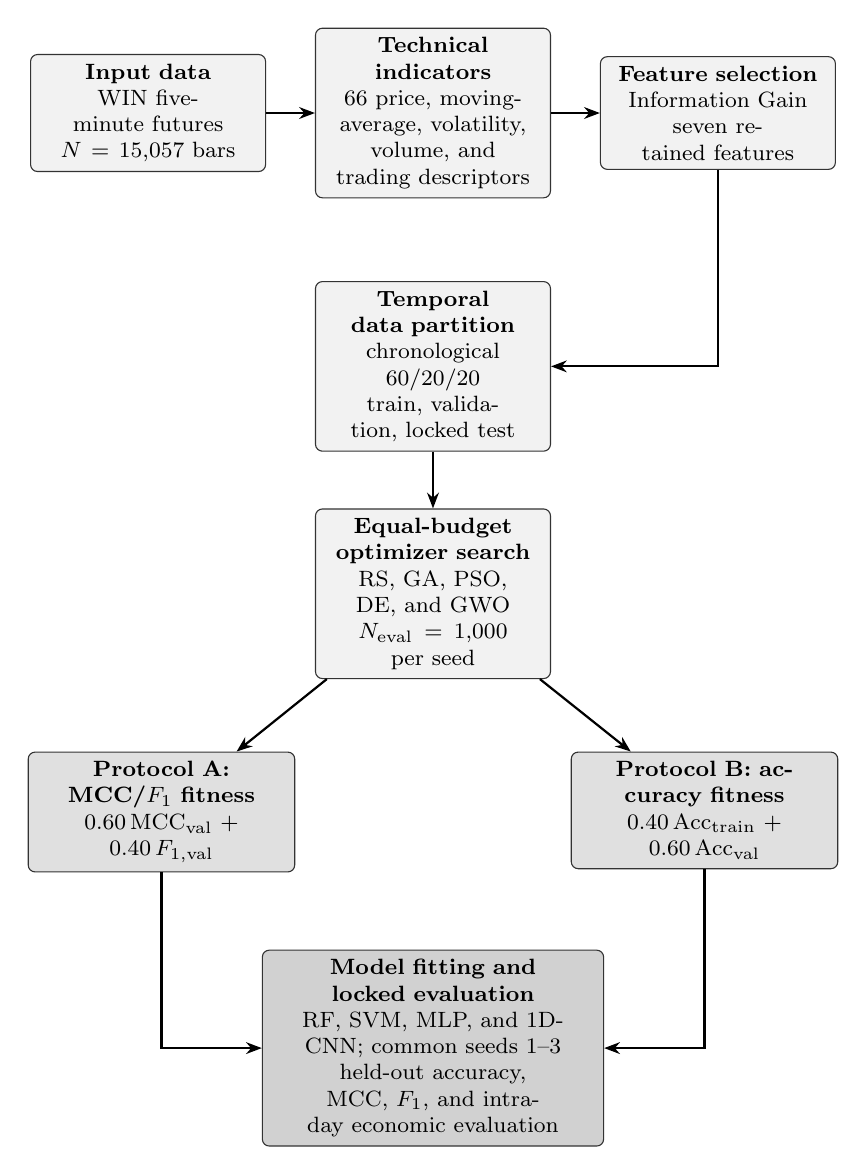
\begin{tikzpicture}[
  node distance=0.72cm and 0.62cm,
  every node/.style={
    draw=black!80,
    rounded corners=2.5pt,
    align=center,
    minimum height=0.88cm,
    text width=2.75cm,
    font=\footnotesize
  },
  process/.style={fill=black!5},
  protocol/.style={fill=black!12, text width=3.15cm},
  outcome/.style={fill=black!18, text width=4.10cm},
  arrow/.style={-{Stealth[length=2.0mm]}, thick}
]
  \node[process] (data) {\textbf{Input data}\\WIN five-minute futures\\$N=15{,}057$ bars};
  \node[process, right=of data] (indicators) {\textbf{Technical indicators}\\66 price, moving-average, volatility, volume, and trading descriptors};
  \node[process, right=of indicators] (selection) {\textbf{Feature selection}\\Information Gain\\seven retained features};

  \node[process, below=1.05cm of indicators] (split) {\textbf{Temporal data partition}\\chronological 60/20/20\\train, validation, locked test};
  \node[process, below=of split] (search) {\textbf{Equal-budget optimizer search}\\RS, GA, PSO, DE, and GWO\\$N_{\mathrm{eval}}=1{,}000$ per seed};

  \node[protocol, below left=0.92cm and 0.25cm of search] (mcc) {\textbf{Protocol A: MCC/$F_1$ fitness}\\$0.60\,\mathrm{MCC}_{\mathrm{val}}+0.40\,F_{1,\mathrm{val}}$};
  \node[protocol, below right=0.92cm and 0.25cm of search] (accuracy) {\textbf{Protocol B: accuracy fitness}\\$0.40\,\mathrm{Acc}_{\mathrm{train}}+0.60\,\mathrm{Acc}_{\mathrm{val}}$};
  \coordinate (protocolmid) at ($(mcc.south)!0.5!(accuracy.south)$);
  \node[outcome, below=1.00cm of protocolmid] (test) {\textbf{Model fitting and locked evaluation}\\RF, SVM, MLP, and 1D-CNN; common seeds 1--3\\held-out accuracy, MCC, $F_1$, and intraday economic evaluation};

  \draw[arrow] (data) -- (indicators);
  \draw[arrow] (indicators) -- (selection);
  \draw[arrow] (selection.south) |- (split.east);
  \draw[arrow] (split) -- (search);
  \draw[arrow] (search) -- (mcc);
  \draw[arrow] (search) -- (accuracy);
  \draw[arrow] (mcc.south) |- (test.west);
  \draw[arrow] (accuracy.south) |- (test.east);
\end{tikzpicture}%
}
\caption{Overview of the proposed methodology. The pipeline retains the precursor's sequence of intraday data preparation, indicator construction, feature selection, model fitting, and final evaluation; the new benchmark inserts a chronological partition, equal-budget optimizer comparison, and two explicitly separated validation objectives.}
\label{fig:workflow}
\end{figure}

\begin{figure}[htbp]
\centering
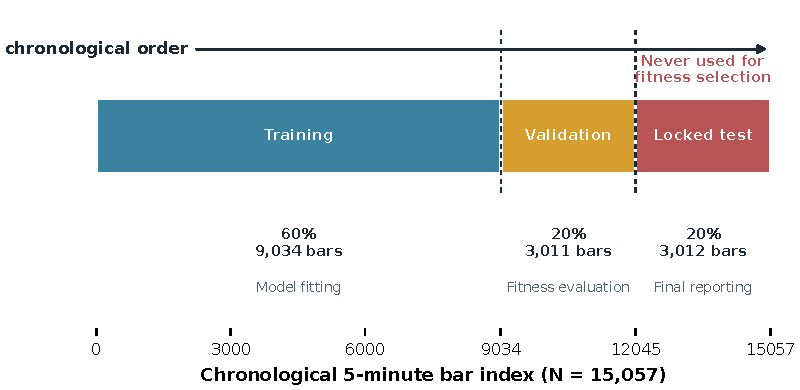
\includegraphics[width=0.86\linewidth]{figures/dual_fitness_temporal_split.pdf}
\caption{Chronological 60/20/20 partition. The final test block is unavailable during feature fitting, candidate ranking, and hyperparameter selection.}
\label{fig:temporal_split}
\end{figure}

\subsection{Evidence Scope, Statistical Analysis, and Economic Evaluation}

Three seeds (1--3) are available for every model--optimizer combination in both protocols. Therefore, the direct protocol contrast uses 20 cell means per protocol, each averaged over the same three seeds, and is presented descriptively. It is not a 20-seed confirmatory test of one fitness against another.

A complementary model-level analysis is performed within each holdout protocol. The five optimizer--seed combinations form 15 matched blocks for the four model backbones. Friedman tests assess global rank differences, followed by paired Wilcoxon tests with Holm adjustment for post-hoc MLP contrasts. This analysis answers whether models separate within a fixed protocol; it does not infer a global fitness advantage.

Finally, the locked predictions are evaluated through an intraday long/short trading simulation. The analysis reports total profit, profit factor, annualized Sharpe ratio, and maximum drawdown. Economic results are interpreted jointly with predictive metrics because a trading strategy can have different return and drawdown characteristics despite similar classification accuracy.

\section{Results}\label{sec:results}

\subsection{Predictive Outcomes Under Two Selection Objectives}

Figure~\ref{fig:paired_outcomes} reports held-out accuracy and MCC for the 20 model--optimizer cells. Each line connects a cell evaluated under the two fitness functions and is averaged over the same three seeds. Across cells, the descriptive macro mean test accuracy is 0.623 for MCC/$F_1$ fitness and 0.617 for accuracy fitness. The corresponding macro mean test MCC values are 0.247 and 0.235. These quantities summarize the available cells; they are not population estimates.

The result is informative because it rejects a simplistic expectation that selecting on validation accuracy must increase every held-out accuracy value. Some configurations improve under accuracy fitness, whereas others decline, and the corresponding MCC changes are likewise heterogeneous. The selection objective thus interacts with backbone and optimizer rather than imposing a uniform ordering.

\begin{figure}[htbp]
\centering
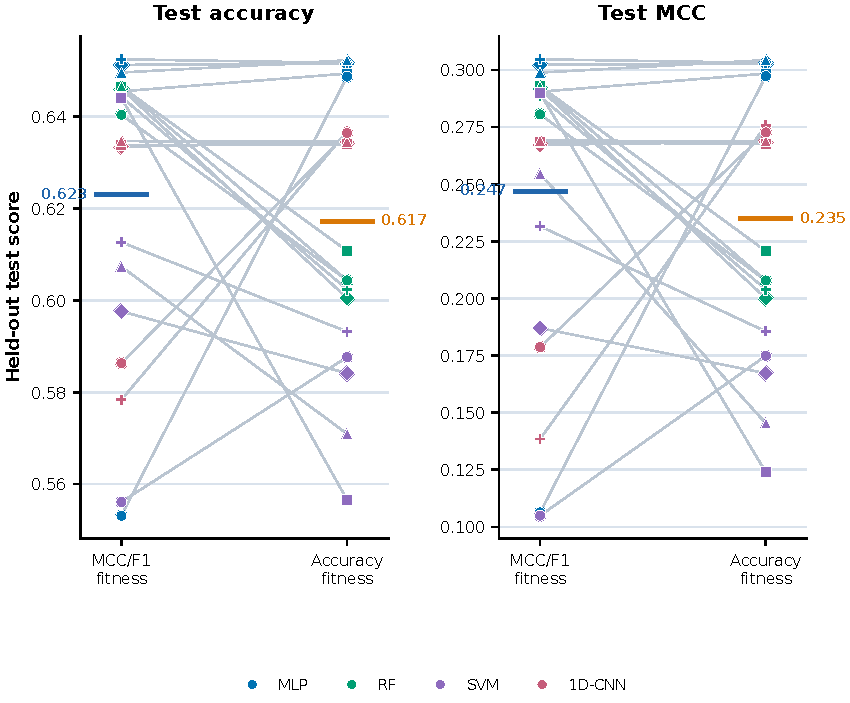
\includegraphics[width=0.96\linewidth]{figures/dual_fitness_paired_outcomes.pdf}
\caption{Held-out test outcomes under the two validation objectives. Each connection is one model--optimizer cell averaged over paired seeds 1--3. Colour denotes the model backbone; marker shape denotes the optimizer. Horizontal segments show macro means across the 20 cells.}
\label{fig:paired_outcomes}
\end{figure}

Figure~\ref{fig:delta_heatmaps} localizes the contrast by model and optimizer. Positive cells favour accuracy fitness and negative cells favour compound MCC/$F_1$ fitness. The heterogeneity reinforces the need to distinguish a selection objective from a reported test metric and motivates a larger common-seed study before making global superiority claims.

\begin{figure}[htbp]
\centering
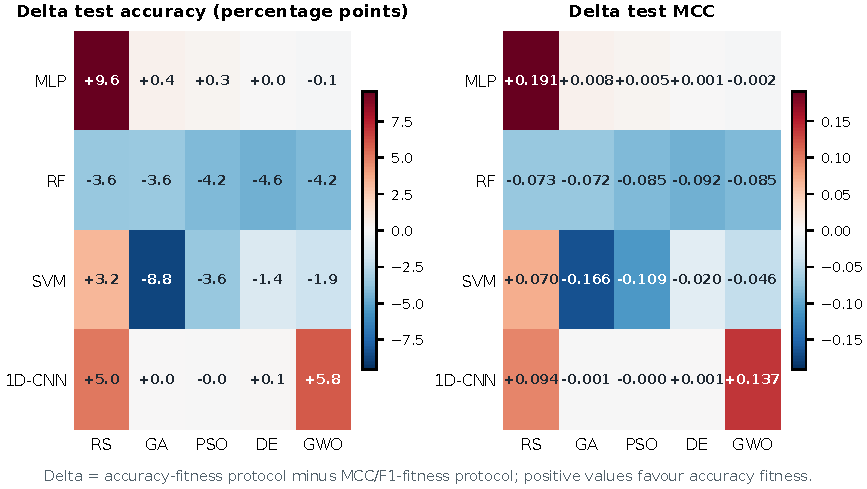
\includegraphics[width=0.96\linewidth]{figures/dual_fitness_delta_heatmaps.pdf}
\caption{Configuration-level difference between protocols (accuracy fitness minus MCC/$F_1$ fitness) on the locked test set. Left: accuracy in percentage points. Right: MCC in raw units.}
\label{fig:delta_heatmaps}
\end{figure}

\subsection{Search Dynamics}

Figure~\ref{fig:convergence} uses MLP as a reference backbone to visualize the objective being optimized. The left panel follows compound MCC/$F_1$ validation fitness, while the right panel follows validation accuracy. The vertical scales differ by construction and must not be interpreted as a direct score comparison. The trajectories show the progress of each optimizer under its assigned objective and make the distinction between the two experiments explicit.

\begin{figure}[htbp]
\centering
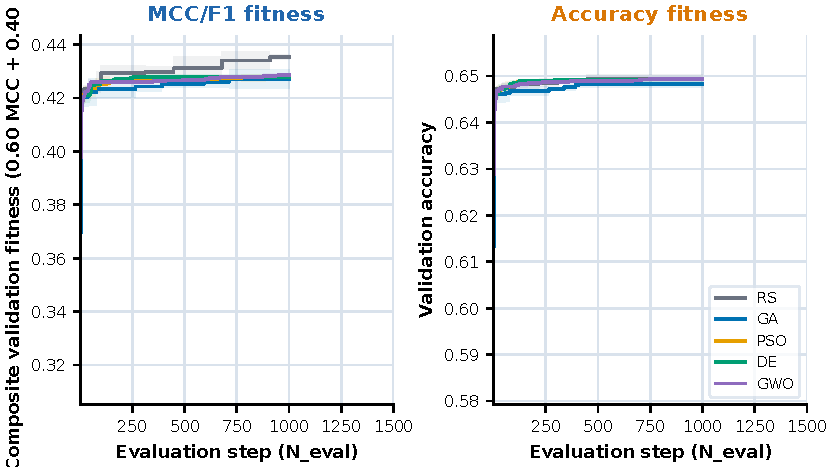
\includegraphics[width=0.96\linewidth]{figures/dual_fitness_convergence.pdf}
\caption{MLP convergence under the two validation objectives. Lines are means and shaded regions are $\pm1$ standard deviation across paired seeds 1--3. Left: compound MCC/$F_1$ fitness. Right: validation accuracy.}
\label{fig:convergence}
\end{figure}

\subsection{Exploratory Statistical Evidence}

Within Protocol A, the Friedman comparison across 15 matched optimizer--seed blocks identifies differences in test MCC among the four model backbones ($\chi^2=22.84$, $p=4.36\times10^{-5}$). Within Protocol B, the analogous test on accuracy is also significant ($\chi^2=42.92$, $p=2.56\times10^{-9}$), with MLP receiving mean rank 1.00. In Protocol B, Holm-adjusted MLP contrasts are significant against CNN, RF, and SVM ($p_{\mathrm{Holm}}=0.00194$ in each comparison).

These tests are exploratory and model-level. They do not test MCC/$F_1$ fitness against accuracy fitness, and their 15 blocks should not be confused with 15 independent market periods. Figure~\ref{fig:statistical_summary} makes this scope visible.

\begin{figure}[htbp]
\centering
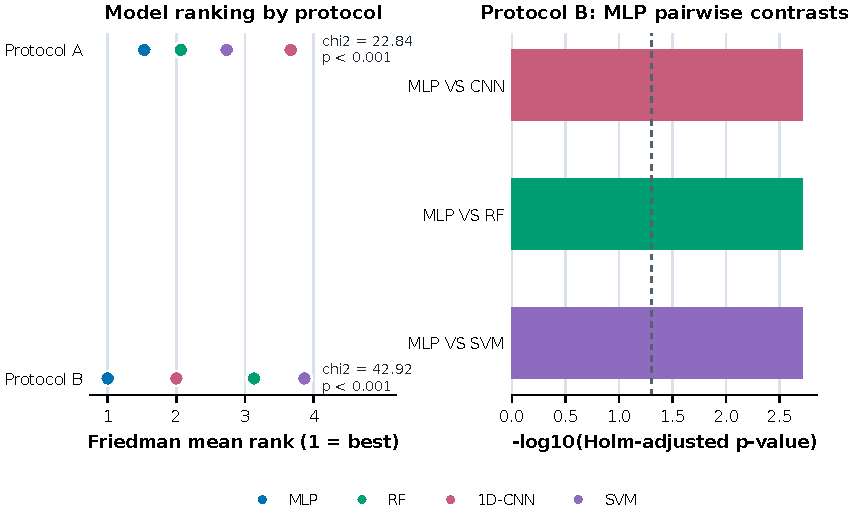
\includegraphics[width=0.96\linewidth]{figures/dual_fitness_statistical_summary.pdf}
\caption{Exploratory statistical evidence within each holdout protocol. Left: Friedman mean ranks across 15 matched optimizer--seed blocks (lower is better). Right: Holm-adjusted paired Wilcoxon evidence for MLP versus the other models under accuracy fitness; the dashed line denotes $\alpha=0.05$.}
\label{fig:statistical_summary}
\end{figure}

\subsection{Economic Evaluation}

The economic evaluation reveals a related but distinct ranking. Under MCC/$F_1$ fitness, RF has the largest mean total profit (26,465 points), but its Holm-adjusted profit contrasts are not significant. Under accuracy fitness, MLP has the largest mean total profit (27,737 points). MLP's profit advantage is significant against RF ($p_{\mathrm{Holm}}=0.00018$) and SVM ($p_{\mathrm{Holm}}=0.00305$), but not against CNN ($p_{\mathrm{Holm}}=0.169$). RF has the least negative mean drawdown under accuracy fitness ($-1,866$ points).

Figure~\ref{fig:economic_summary} shows why accuracy alone is insufficient for selection: total profit, dispersion, and drawdown do not always identify the same preferred configuration. The comparison is exploratory but establishes the economic endpoint absent from the precursor study.

\begin{figure}[htbp]
\centering
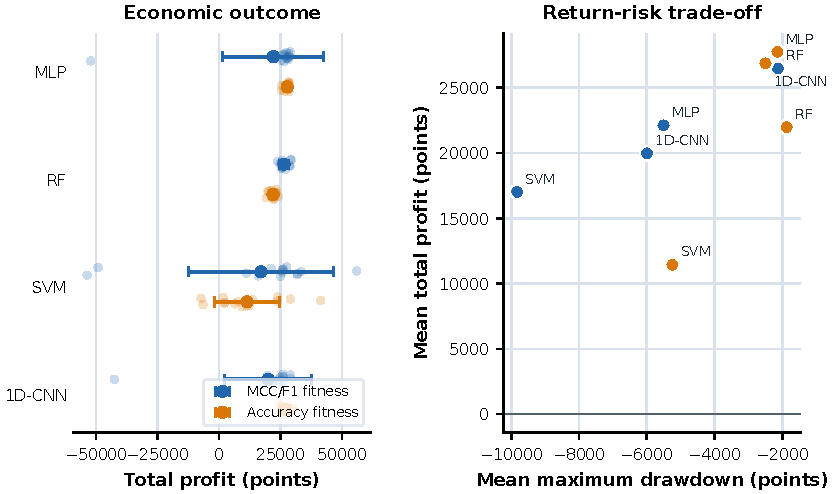
\includegraphics[width=0.96\linewidth]{figures/dual_fitness_economic_summary.pdf}
\caption{Exploratory economic evaluation on the locked test block. Left: total-profit observations and mean $\pm1$ standard deviation across 15 optimizer--seed blocks. Right: mean profit versus mean maximum drawdown; values farther right have less severe drawdown.}
\label{fig:economic_summary}
\end{figure}

\section{Discussion}\label{sec:discussion}

The main advance over the GA-based precursor is methodological control. The earlier work offered a useful proof of concept for combining technical indicators, feature selection, and GA tuning, but it could not distinguish optimizer behaviour from the consequences of randomized validation and unequal search opportunity. The present design makes these assumptions visible: chronological data ordering is preserved, evaluation budgets are fixed, and the validation criterion is stated separately from the final test metrics.

The direct comparison does not support a simple rule that accuracy fitness should dominate when accuracy is reported, or that MCC/$F_1$ fitness should dominate every robust metric. The paired cells show positive and negative changes under each criterion. This is plausible in intraday markets, where validation performance is affected by small decision-boundary changes and the final chronological block may represent a different regime. For this reason, the appropriate interpretation is objective-dependent behaviour, not a universal ranking of the two fitness functions.

The within-protocol exploratory analysis provides a more bounded result. MLP ranks first under the accuracy-fitness protocol across matched optimizer--seed blocks, and its adjusted pairwise contrasts against the other backbones are significant. The economic analysis, however, demonstrates that the predictive ordering does not settle the decision alone: RF attains the smallest mean drawdown under accuracy fitness, whereas MLP obtains the largest mean profit. A deployment decision must therefore specify whether return, downside risk, turnover, or stability is the governing criterion.

Several limitations should guide interpretation. Only three seeds are common to all model--optimizer cells in both protocols. The direct dual-fitness results are therefore descriptive, and the model-level Friedman/Wilcoxon analyses are exploratory. The data cover one liquid Brazilian futures market and one chronological test segment; results may differ across instruments and regimes. Finally, the fixed 1,000-evaluation allowance is appropriate for a controlled benchmark but does not reveal long-budget asymptotic behaviour.

The next study phase is clear: run a preregistered common 20-seed design for every cell, retain the same temporal split and candidate budget, record all validation metrics at each candidate evaluation, and apply paired tests separately to MCC, accuracy, and economic outcomes. That extension would permit confirmatory inference about fitness choice while preserving the methodological strengths established here.

\section{Conclusion}\label{sec:conclusion}

This study transforms a GA-based conference precursor into a controlled Neural Computing and Applications benchmark for neural intraday trend classification. It preserves the predecessor's practical insight---a compact, Information-Gain-selected technical representation can support metaheuristic hyperparameter search---but replaces randomized validation and a single-optimizer design with a chronological dual-fitness protocol, five budget-matched optimizers, and locked predictive and economic assessment.

The current evidence indicates that the choice between compound MCC/$F_1$ fitness and accuracy fitness produces configuration-dependent changes in both held-out accuracy and MCC. Within the accuracy-fitness protocol, MLP is the strongest model in the exploratory predictive analysis and leads mean total profit, although RF has the smallest mean drawdown. These results reinforce the central methodological lesson: selection objective, reported metric, and economic utility must be treated as related but distinct quantities.

The manuscript deliberately avoids a confirmatory claim about a universal best fitness function because only three paired seeds are currently available across every cell. Completing the common 20-seed design is the necessary next step. The resulting framework nevertheless provides a transparent and reproducible basis for future optimizer comparisons in non-stationary financial time series.

% ============================================================
% Declarations
% Mirror: Al Bannoud et al. (NCA 2026) Declarations section
% ============================================================

\section*{Declarations}

\subsection*{Funding}
This study was financed in part by the Coordena\c{c}\~{a}o de Aperfei\c{c}oamento de Pessoal de N\'{\i}vel Superior -- Brasil (CAPES) -- Finance Code 001.

\subsection*{Conflict of Interest}
The authors declare that they have no conflict of interest or competing financial interests.

\subsection*{Ethical Approval}
This article does not contain any studies with human participants or animals performed by any of the authors.

\subsection*{Data and Code Availability}
The datasets generated and analyzed during the current study, along with the complete source code for all optimization algorithms, benchmark scripts, and evaluation pipelines, are available in the project repository upon reasonable request.

\subsection*{Author Contributions}
All authors contributed to the study conception and design. Data collection and experimental execution were performed by [Anonymous for double-blind review]. Statistical analysis and manuscript preparation were carried out by [Anonymous for double-blind review]. All authors read and approved the final manuscript.


\bibliography{references}
\end{document}
